\begin{pastexam}[label={px:ntu-114-bime-ds-03}]{臺大生機所 114 學年度 第 3 題}
（追蹤、計算；共 20 分）

\textbf{(10\%)} Construct a max-oriented heap by inserting the keys E, A, S, Y, Q, U, E, S, T, I, O,
N into an initially empty heap in the given order. Provide the final heap represented as an array
after all the keys have been inserted.\\
\textbf{(5\%)} Determine the time complexity of inserting an element into a max-oriented heap.
Specifically, analyze the insertion process, considering how the heap property is maintained after
the insertion.\\
\textbf{(5\%)} Determine the amortized time complexity of inserting an element in to the
max-oriented heap when a resized array is used. Assume the following resizing rule: when the array
becomes full, it is resized by doubling its current size.
\end{pastexam}

\begin{pastsoln}
本題的三小題依序記為 (a)(b)(c)。 (a)(b) 屬資結書第~8~章，(c) 是第~3.4~節的平攤分析。

\textbf{(a)} 鍵值是字母，照字母順序比大小（$\mathrm{A} < \mathrm{E} < \cdots < \mathrm{Y}$）。 陣列
從第 $1$ 格開始放，節點 $i$ 的父節點是 $\lfloor i/2 \rfloor$。 插入的做法（資結書虛擬碼~8.2）：
新鍵值放在最後一格，只要比父節點\textbf{大}就和父節點交換，相等不交換。

\begin{center}
\small
\begin{tabular}{cccl}
\toprule
插入 & 放在 & 和誰交換（格號） & 插入後的陣列（第 $1$ 格起） \\
\midrule
E & 1 & -- & E \\
A & 2 & -- & E A \\
S & 3 & E(1) & S A E \\
Y & 4 & A(2)，S(1) & Y S E A \\
Q & 5 & --（Q $<$ S） & Y S E A Q \\
U & 6 & E(3) & Y S U A Q E \\
E & 7 & --（E $<$ U） & Y S U A Q E E \\
S & 8 & A(4)；再比 S(2)，相等，停 & Y S U S Q E E A \\
T & 9 & S(4)，S(2)；Y 比較大，停 & Y T U S Q E E A S \\
I & 10 & --（I $<$ Q） & Y T U S Q E E A S I \\
O & 11 & --（O $<$ Q） & Y T U S Q E E A S I O \\
N & 12 & E(6)；U 比較大，停 & Y T U S Q N E A S I O E \\
\bottomrule
\end{tabular}
\end{center}

最後的堆積：
\begin{center}
\begin{tabular}{c*{12}{c}}
\toprule
格號 & 1 & 2 & 3 & 4 & 5 & 6 & 7 & 8 & 9 & 10 & 11 & 12 \\
\midrule
鍵值 & Y & T & U & S & Q & N & E & A & S & I & O & E \\
\bottomrule
\end{tabular}
\end{center}
\begin{center}
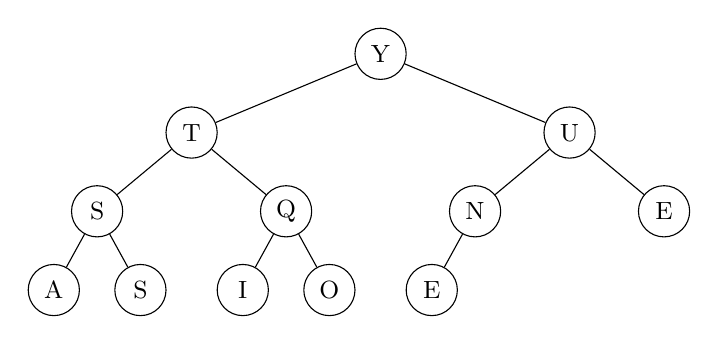
\begin{tikzpicture}[every node/.style={circle,draw,minimum size=6.5mm,inner sep=0pt,font=\small},
  level distance=10mm, level 1/.style={sibling distance=48mm}, level 2/.style={sibling distance=24mm},
  level 3/.style={sibling distance=11mm}]
\node {Y}
  child {node {T} child {node {S} child {node {A}} child {node {S}}}
                  child {node {Q} child {node {I}} child {node {O}}}}
  child {node {U} child {node {N} child {node {E}} child[missing]}
                  child {node {E}}};
\end{tikzpicture}
\end{center}
檢查：每個節點都不小於子節點（例如 T 的子節點 S、Q；N 的子節點 E）。

\textbf{(b)} 插入分兩步：
\begin{enumerate}
\item 把新元素放在陣列最後一格（第 $n + 1$ 格），樹仍然是完整二元樹，$O(1)$。
\item 唯一可能違反堆積性質的是新元素和它父節點之間。 新元素比父節點大就交換，交換後原來的
父節點換到下面，它本來就不小於那個位置的其他子孫，所以問題只會往上移一層；一直做到父節點不比
它小或到了根。 每一層做一次比較、最多一次交換。
\end{enumerate}
$n$ 個元素的完整二元樹有 $\lfloor \lg n \rfloor + 1$ 層（資結書定理~7.3），新元素從最底層往上最多
走 $\lfloor \lg n \rfloor$ 層，所以插入是 $O(\log n)$。 最壞情況是新元素比全部都大，要一路換到根，$\Theta(\log n)$；最好情況是
它不比父節點大，$O(1)$。

\textbf{(c)} 用加倍的可變大小陣列：容量 $c$ 用完時，配置大小 $2c$ 的新陣列、把 $c$ 個元素複製過去
（$c$ 次搬移），再插入。 用聚合分析（資結書第~3.4~節）：從容量 $1$ 開始連續插入 $n$ 個元素，
擴充發生在第 $1, 2, 4, \ldots, 2^{k}$ 次插入之後（$2^{k} < n$），搬移總數
\[
1 + 2 + 4 + \cdots + 2^{k} = 2^{k+1} - 1 < 2n .
\]
所以擴充的成本平攤到每次插入是 $O(1)$。 每次插入另外要做 (b) 的往上調整，最多
$O(\log n)$。 總和：
\[
n \text{ 次插入的總時間} \le 2n + \sum_{i=1}^{n} O(\log i) = O(n \log n),
\]
\textbf{平攤每次插入 $O(\log n)$}；其中陣列擴充只貢獻平攤 $O(1)$，並沒有讓插入變慢。 注意單獨
一次插入碰上擴充時要 $\Theta(n)$，加倍的好處是這種貴的操作很少，平攤下來不影響。 （若改成每次
只多加固定 $k$ 格，搬移總數是 $\Theta(n^2/k)$，平攤每次 $\Theta(n)$。）
\end{pastsoln}
